\documentclass{article}
\usepackage{titlesec}
\usepackage[utf8]{inputenc}
\usepackage[a4paper, total={6in, 9in}]{geometry}
\usepackage{fancyhdr}
\usepackage{graphicx} % Add the graphicx package
\usepackage{lipsum} % For placeholder text
\usepackage{tikz}
\usepackage{cite}
\usepackage{bm}
\usepackage{acronym}
\usepackage{amsmath,amssymb,amsfonts}
\usepackage{algorithmic}
\usepackage{graphicx}
\usepackage{caption}
\usepackage{subcaption}
\captionsetup{font=small, labelfont=bf}
\captionsetup[sub]{labelsep=period, subrefformat=brace}
\usepackage{tikz}
\usepackage{textcomp}
\usepackage{xcolor}
\usepackage[numbers]{natbib}
\bibliographystyle{ieeetrann}
\usepackage{subfig}
\usepackage{svg}
\usepackage{tikz,pgfplots,pgfplotstable}
\usepackage{subfigure}
\usetikzlibrary{matrix, positioning, arrows.meta}
\usepackage{multirow}
\usepackage{listings}
\usepackage{xcolor}

\definecolor{codegreen}{rgb}{0,0.6,0}
\definecolor{codegray}{rgb}{0.5,0.5,0.5}
\definecolor{codepurple}{rgb}{0.58,0,0.82}
\definecolor{backcolour}{rgb}{0.95,0.95,0.92}

\lstdefinestyle{mystyle}{
    backgroundcolor=\color{backcolour},   
    commentstyle=\color{codegreen},
    keywordstyle=\color{magenta},
    numberstyle=\tiny\color{codegray},
    stringstyle=\color{codepurple},
    basicstyle=\ttfamily\footnotesize,
    breakatwhitespace=false,         
    breaklines=true,                 
    captionpos=b,                    
    keepspaces=true,                 
    numbers=left,                    
    numbersep=5pt,                  
    showspaces=false,                
    showstringspaces=false,
    showtabs=false,                  
    tabsize=2
}

\lstset{style=mystyle}

\usepackage[
backend=biber,
style=numeric,
sorting=none
]{biblatex}

\addbibresource{references.bib}

\title{Bibliography management: \texttt{biblatex} package}
\author{Share\LaTeX}
\date{08/03/2024}


% Set up page headers and footers
\pagestyle{fancy}
\fancyhf{}
\rhead{ }
\lhead{UART Implementation}
\cfoot{\thepage}

% Redefine the abstract environment to be single column
\renewenvironment{abstract}
{\par\noindent\textbf{\abstractname}\ \ignorespaces}{\par}

% Redefine section format
\titleformat{\section}
{\normalfont\Large\bfseries}{\thesection}{1em}{}

\begin{document}
	
	% Cover Page
	\begin{titlepage}
		
		\centering
		\vspace*{0.5cm}
		
\includegraphics[width=5cm]{logo.png} % Replace with the path to your university logo
		\par\vspace{0.02cm}
		Department of Electronic \& Telecommunication Engineering
  
            University of Moratuwa, Sri Lanka.
		\par\vspace{4cm}
		{\LARGE\bfseries UART Implementation\par}
		\vspace{5cm}
		\begin{tabular}{c c}
			& \\
            210608J &   Silva L.J.J.P.\\
            210609M	&	Silva M.K.Y.U.N.\\
            210610H &   Sirimanna N.T.W.\\
		\end{tabular}\\
		\vspace{1.3cm}
            {Submitted in partial fulfillment of the requirements for the module\par}
		{EN 2111 Electronic Circuit Design\par}
	
		\vspace{0.5cm}
		{\large 05/08/2024\par}
		\vfill
	\end{titlepage}
	
	\newpage       
            \tableofcontents
            
	\newpage
            \section{What is UART?}
                UART, or universal asynchronous receiver-transmitter, is one of the most widely used device-to-device communication protocols. UART is a hardware communication protocol that uses asynchronous serial communication with configurable speed. Asynchronous means that there is no clock signal to synchronise the transmitting device's output bits as they travel to the receiving end.\\
                    
                When properly configured, UART can work with many different types of serial protocols that involve transmitting and receiving serial data. In serial communication, data is transferred bit by bit using a single line or wire. In two-way communication, we use two wires for successful serial data transfer. Depending on the application and system requirements, serial communications need less circuitry and wires, which reduces the cost of implementation.


                    \begin{enumerate}
                        \item \textbf{Data Framing}: In UART communication, data is sent in packets called frames. Each frame typically consists of a start bit, data bits (usually 8 bits), an optional parity bit for error checking, and one or more stop bits. The start bit signals the beginning of a frame, while the stop bit(s) indicate the end, providing synchronization for the data transmission.
                        
                        \item \textbf{Synchronization}: UART is asynchronous, meaning there is no separate clock signal shared between the transmitter and receiver to synchronize their communication. Instead, both devices must agree on a specific baud rate, which determines the speed at which bits are transmitted and received. The receiver uses the start bit to synchronize with the incoming data stream and then samples the bits at the correct intervals based on the baud rate.
                        
                        \item \textbf{Baud Rate}: The baud rate is the rate at which data is transferred in bits per second (bps). It represents the number of times the signal on the communication line changes state per second. Both the transmitter and receiver must be configured to use the same baud rate for successful communication. Common baud rates include 9600, 19200, 38400, and 115200 bps, among others.

                    \end{enumerate}
                            
                    \section{Phase 1 – Find a Verilog RTL for UART transceiver}

                    \subsection{Baudrate Generator}
                        Following Verilog code defines a baud rate generator module that converts a 50MHz clock into a pair of clocks for transmitting and receiving data at a baud rate of 115200. The receiver clock oversamples by 16x. The module maintains two accumulators, \texttt{rx\_acc} and \texttt{tx\_acc}, to track the number of clock cycles for the receiver and transmitter clocks, respectively. These accumulators are incremented on each positive edge of the 50MHz clock. When either accumulator reaches its maximum value, it resets to zero, ensuring the clocks are synchronized to the desired baud rate. The \texttt{Rxclk\_en} and \text{Txclk\_en} signals indicate when the clocks are enabled for receiving and transmitting data, respectively.\\

                    \lstinputlisting[language=Verilog]{baudTick.v}

                    \subsection{Selected Transmitter Design}
                    
                        The transmitter is deigned to convert the parallel data to serial form using a shift right register and transmit the data over to the receiver maintaining a fixed baud rate. It also consists of a Tx Enable input which is used as a trigger to begin transmission, a reset input to reset the transmission line and bit counter to keep track of the number of bits transferred.
                        
                        \lstinputlisting[language=Verilog]{uartTx.v}

                    \subsection{Selected Receiver Design}
                        The receiver converts the serially received data to a parallel format easy for the computer to process and store. Similar to the Transmitter, this also has a baud counter and a bit counter to synchronise the transmission.

                        
                        \lstinputlisting[language=Verilog]{uartRx.v}

                    \subsection{Transceiver Design}

                    This Verilog module implements a UART transceiver for serial communication. It features components for transmitting and receiving data, utilizing a 50MHz clock. Inputs include data to be transmitted (d\texttt{data\_in}), write enable (\texttt{wr\_en}), clear signal (\texttt{clear}), and receive signal (\texttt{Rx}). Outputs include transmitted data (\texttt{Tx}), busy signal (\texttt{Tx\_busy}), ready signal (\texttt{ready}), received data (\texttt{data\_out}), LED indicators (\texttt{LEDR}), and an extra transmit signal (\texttt{Tx2}). The module interfaces with submodules for baud rate generation, transmitting, and receiving to manage UART functionality.
                    
                        \lstinputlisting[language=Verilog]{uart.v}

                \section{Phase 2 – Develop a Testbench}
                \subsection{Testbench Design}
                    The Testbench is created using Verilog and tests the transciever by connecting the transmitter and receiver to each other and simulate actual communication using random data over a fixed baud rate.
            
                    
                    \lstinputlisting[language=Verilog]{testbench.v}
                    \begin{figure}[!htb]
                        \centering
                            {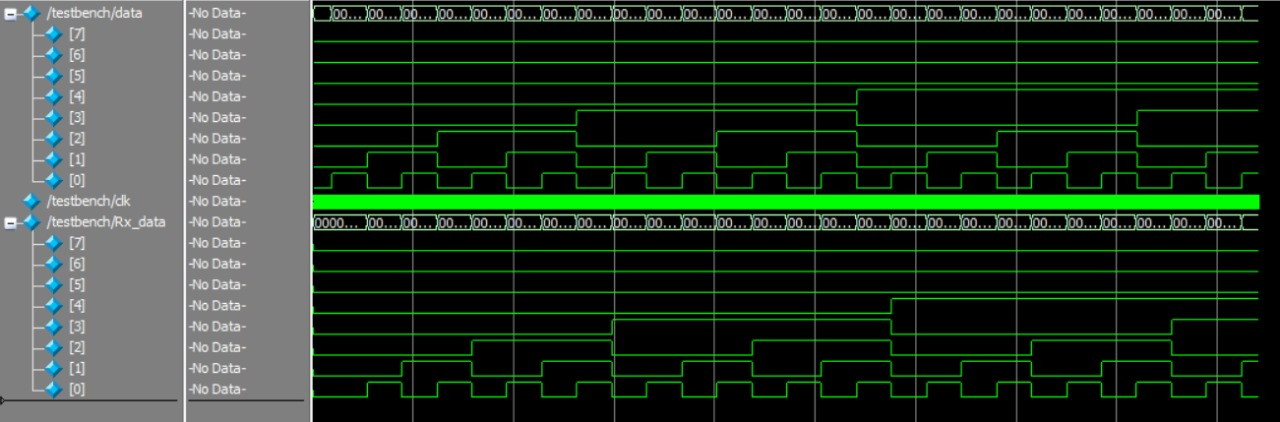
\includegraphics[width=14cm]{wave.jpg}};
                            \caption{Timing Diagram}
                    \end{figure}
                            

                    \section{Phase 3 – Implement RTL Design in FPGA}
                    For this design a DE0-Nano FPGA board was used. On this board, the FPGA chip EP4CE22F17C6N of the family Cyclone IV E has been used. 
                    \begin{figure}[!htb]
                        \centering
                            {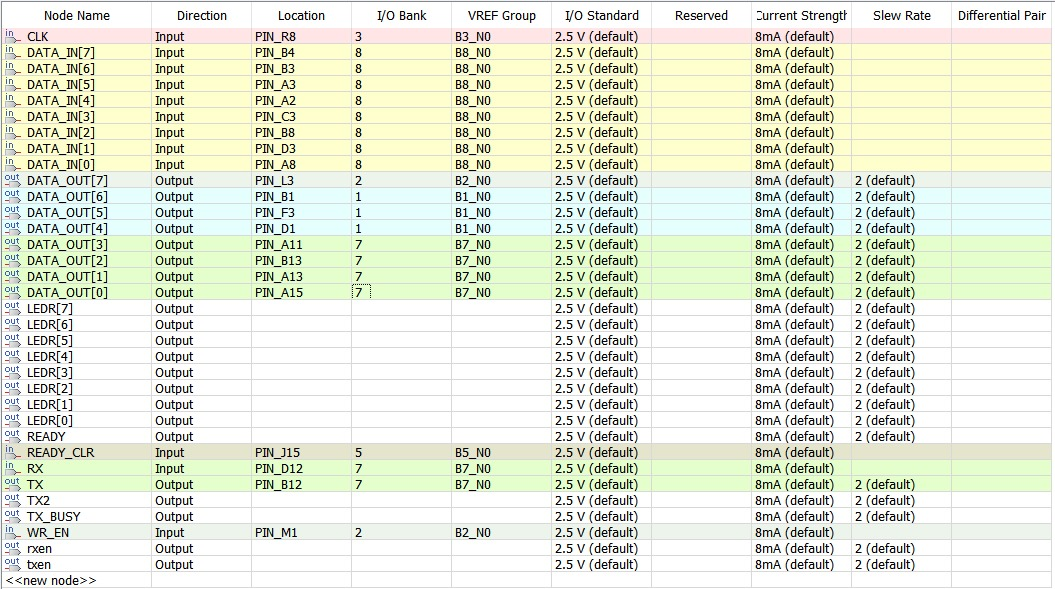
\includegraphics[width=15cm]{pins.jpg}};
                            \caption{Pin Planner pin assignment}
                    \end{figure}

                    The clock signal has been provided from the onboard 50MHz clock. As the data input, we have planned to use the pins 0-7 of the GPIO extension header. To display the data output, we have used the onboard LEDs. To connect with another FPGA board we have used pins 39 (\texttt{RX}) and 40 (\texttt{TX}) on the GPIO pins. For write enable (\texttt{WR\_EN}) we have used one of the onboard DIP switches, and for the \texttt{READY\_CLR} we have used the onboard pushbutton switch. 
\end{document}